%%%%%%%%%%%%%%%%%%%%%%%%%%%%%%%%%%%%%%%%%%%%%%
%                insertmeeting
% 1) Title (something creative & funny?)
% 2) Date (MM/DD/YYYY)
% 3) Location (ex. Hagerty High School)
% 4) People/Committees Present 
% 5) Picture 
% 6) Start Time & Stop Time (ex. 12:30AM to 4:30PM)
%%%%%%%%%%%%%%%%%%%%%%%%%%%%%%%%%%%%%%%%%%%%%%
\insertmeeting 
	{Imperfect Prototyping} 
	{10/07/21}
	{Hagerty High School}
	{Annika, Anouska, Jensen, Nathan, Ritam, Rose, Samantha}
	{Images/RobotPics/robot.jpg}
	{2:30 - 4:30}
	
\subsection*{Hardware}
\noindent\hfil\rule{\textwidth}{.4pt}\hfil
\subsubsection*{Goals}
\begin{itemize}
    \item set up rev hub
    \item build simple arm 

\end{itemize} 

\noindent\hfil\rule{\textwidth}{.4pt}\hfil

\subsubsection*{Accomplishments}
Now that we have the prototype drivetrain built, we decided to continue working and prototyping with it. Because it is constructed out of rev parts, prototyping was far more effiecent than seen with our other designs. Although we have a couple more drivetrain designs we want to build and test, this small 4 wheel tank drive will be fit for most of our basic prototyping. Before we started doing anything else, we needed to get all of the many different electronic components hooked up to the drivetrain. To accomplish this we CADed a middle plate with mounting holes for the Rev hub and battery (Figure \ref{fig:pic1}). From there, we connected the components, downloaded the code and did a test drive.Fortunatley we found that the drivetrain worked very well! The speed was very apparent from the start with this design, which meant that turning was pretty in precise. We started brainstorming about how to make smaller adjustments possible while still preserving the speed. Although we could come up with a software solution, we would have to slow down all of the movement, which will decrease efficiency. One idea we all found enticing was making a car drive. The way a car works is the back wheels are powered and the front wheel pivots, controlling the steering. This would allow us to make fine adjustments while keeping its breakneck speed. Another thing we like about this design is that it is very unique. We are not aware of any team making a drivetrain like this in ftc, so it would differentiate us from all of the other teams this year. To get a better idea of what the drivetrain would look like, we made some sketches we could hand over to the cad committee (Figure \ref{fig:pic2}).
While the cad committee worked on the car drive, we started constructing the arm. The arm connects to the drivetrain with a frame we built out of rev extrusions (Figure \ref{fig:pic3}). After constructing this frame we attached a motor and some bearing brackets. We then used a gear to attach the arm, which is just a long rev extrusion, to the motor. At the end of the arm, we started constructing the first half off our claw. Resembling a spatula (Figure \ref{fig:pic4}), this part of the claw will slide under a block and another part of the claw, which we will construct at a future meeting, will pivot down and clamp a block or ball into the robot.
 

\begin{figure}[ht]
\centering
\begin{minipage}[b]{.50\textwidth}
  \centering
  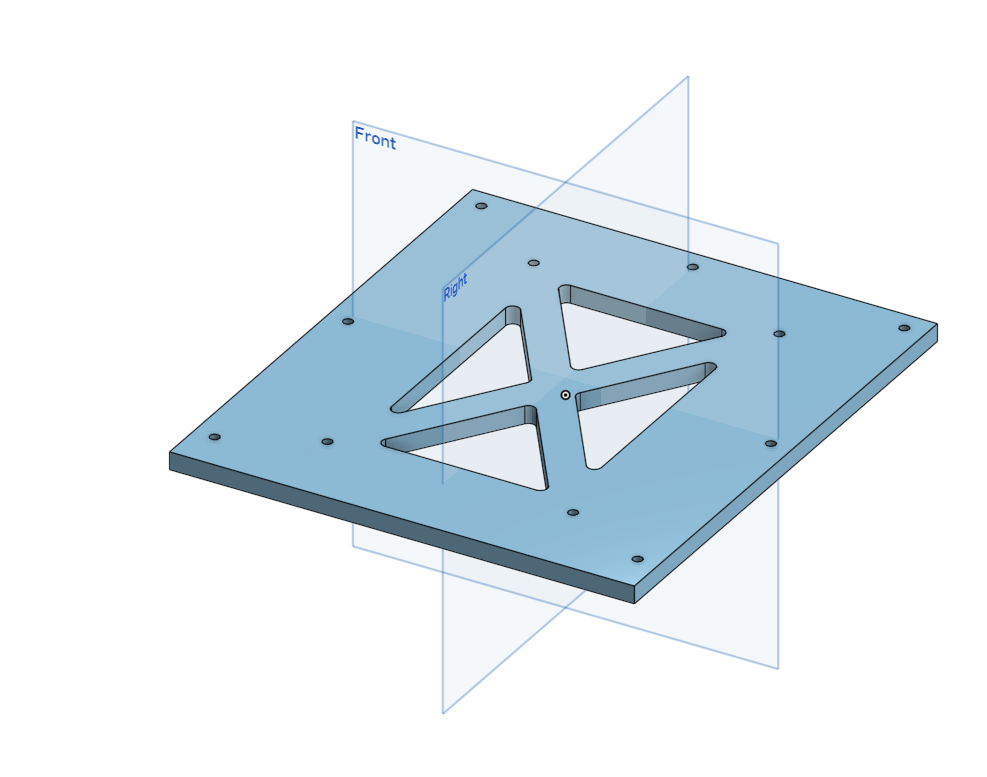
\includegraphics[width=0.8\textwidth]{Meetings/October/10-07-21/10-7-21_Hardware_Figure1 - Nathan Forrer.PNG}
  \caption{Our current RevHub mount with the new holes.}
  \label{fig:pic1}
\end{minipage}%
\hfill%
\begin{minipage}[b]{.50\textwidth}
  \centering
  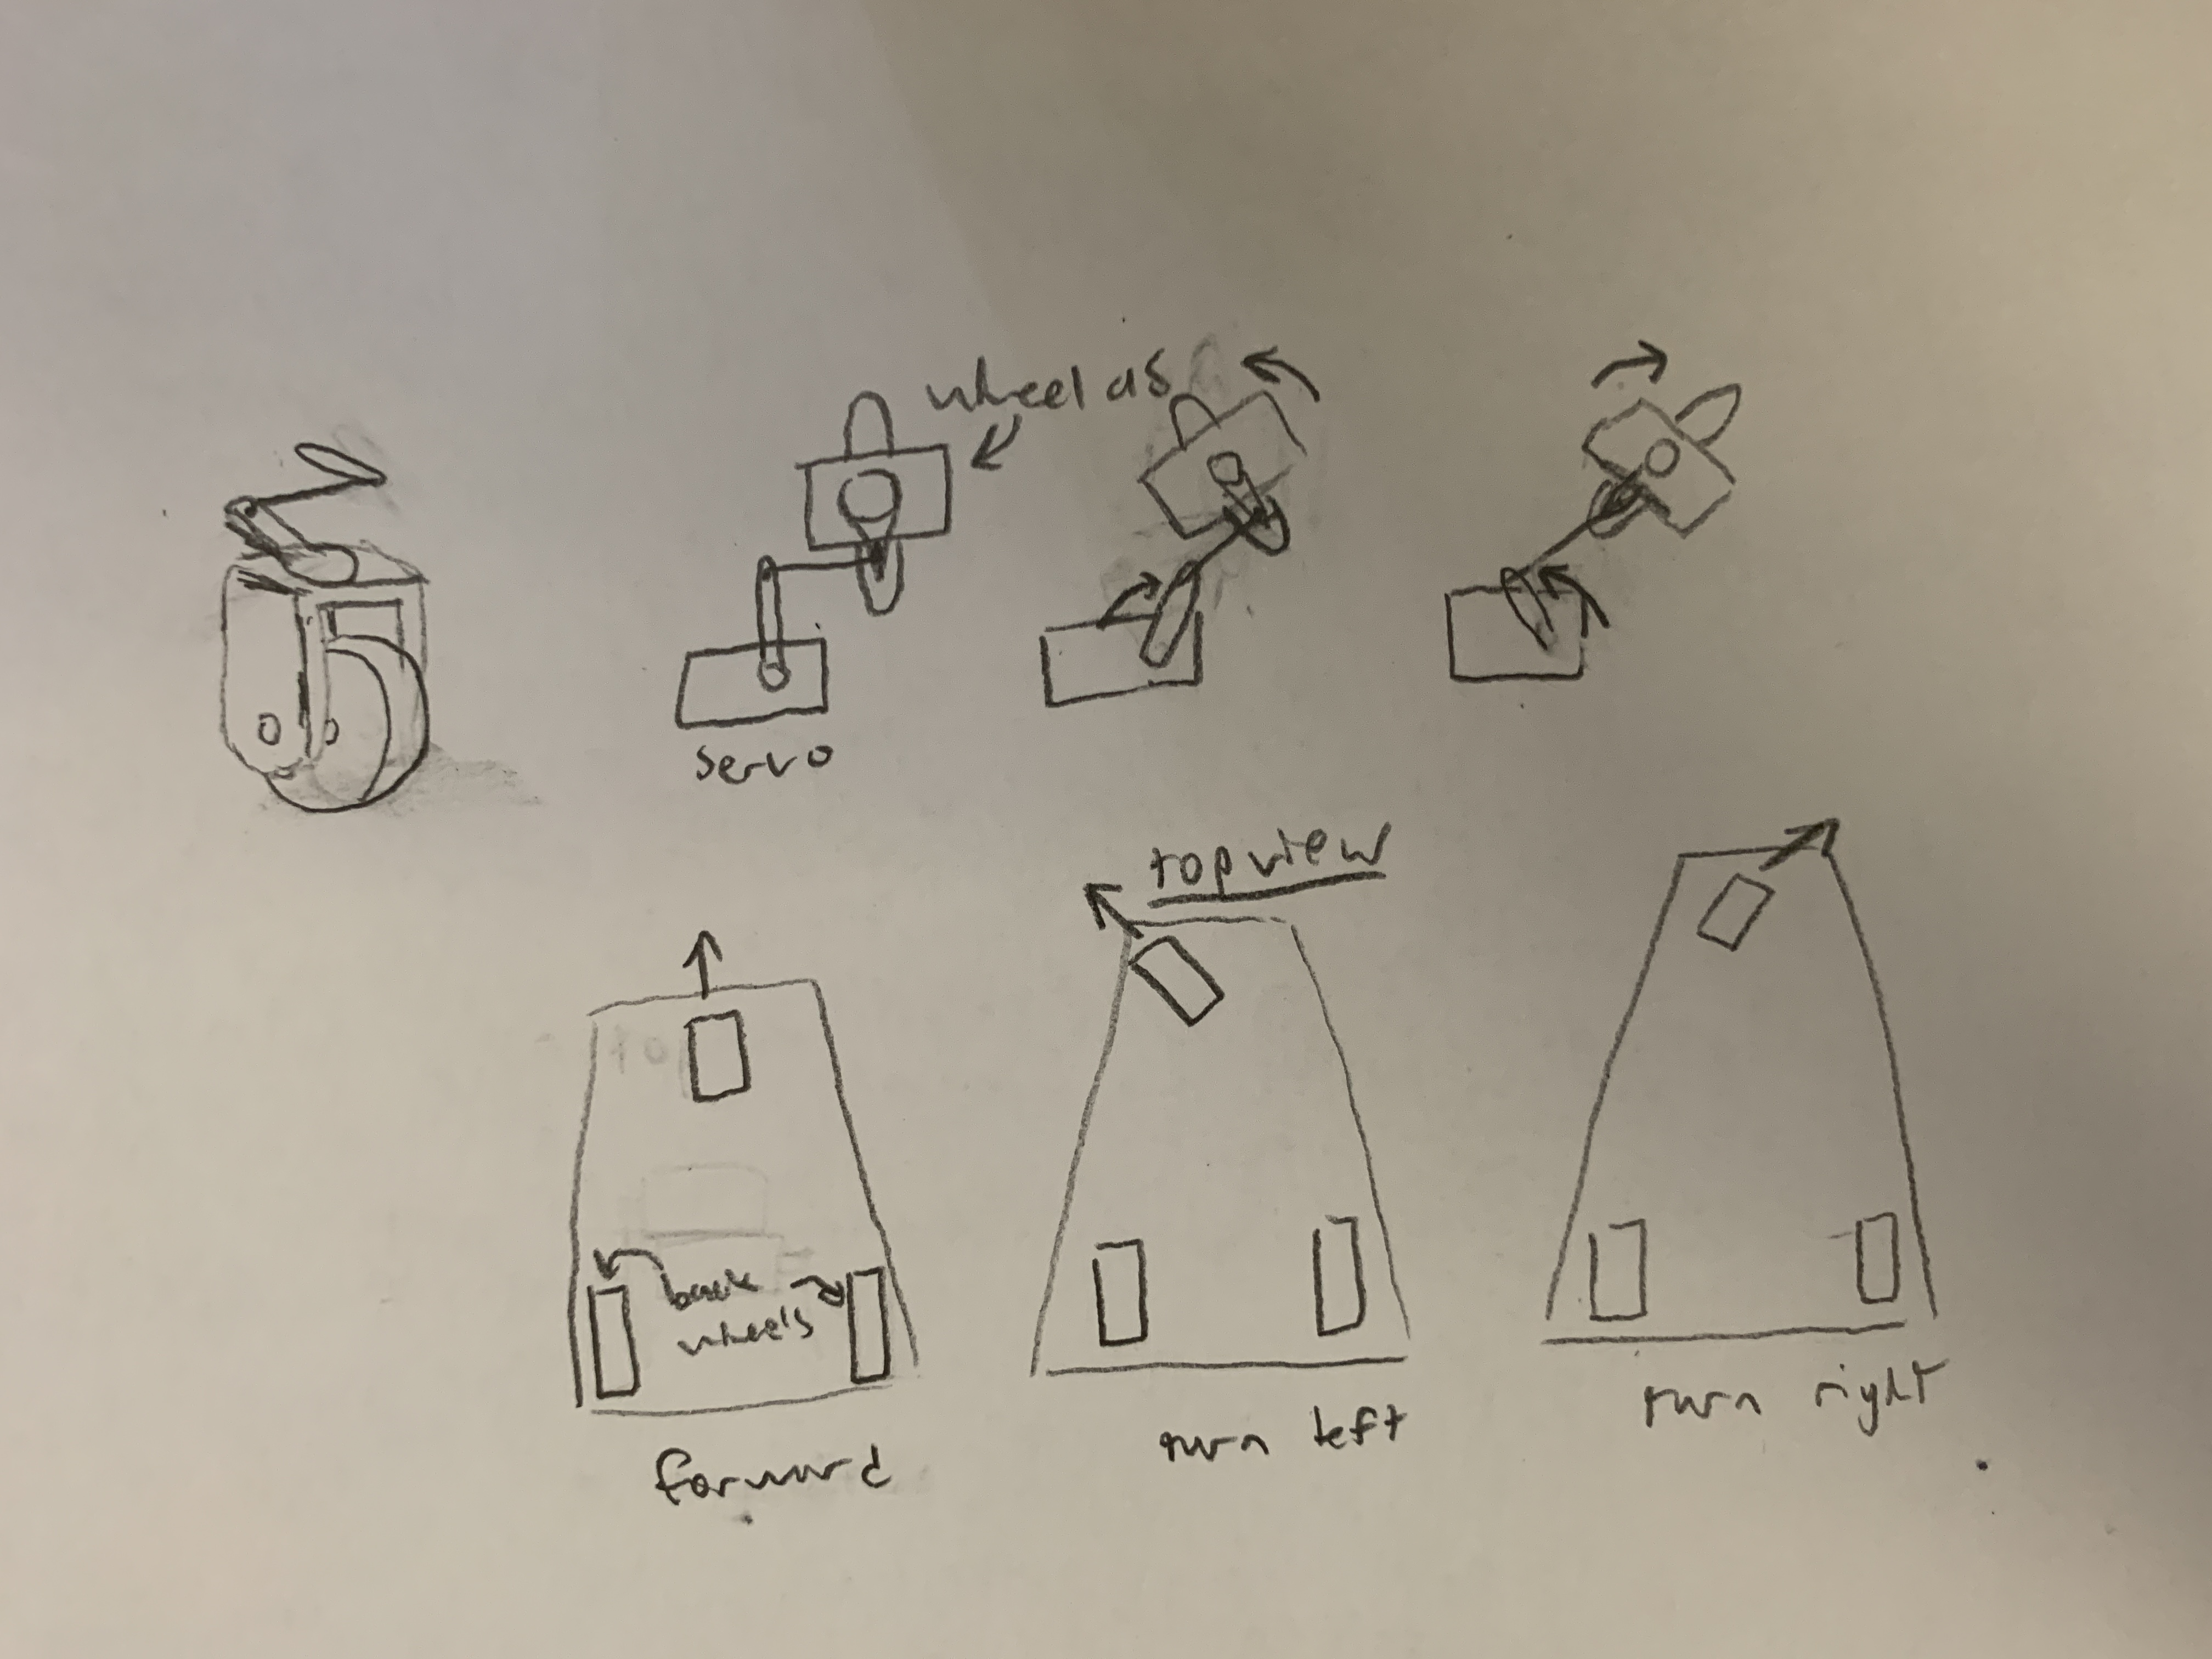
\includegraphics[width=0.8\textwidth]{Meetings/October/10-07-21/10-7-21_Hardware_Figure2 - Nathan Forrer.JPG}
  \caption{Initial sketches of the tricycle drivebase.}
  \label{fig:pic2}
\end{minipage}
\end{figure}

\begin{figure}[ht]
\centering
\begin{minipage}[b]{.50\textwidth}
  \centering
  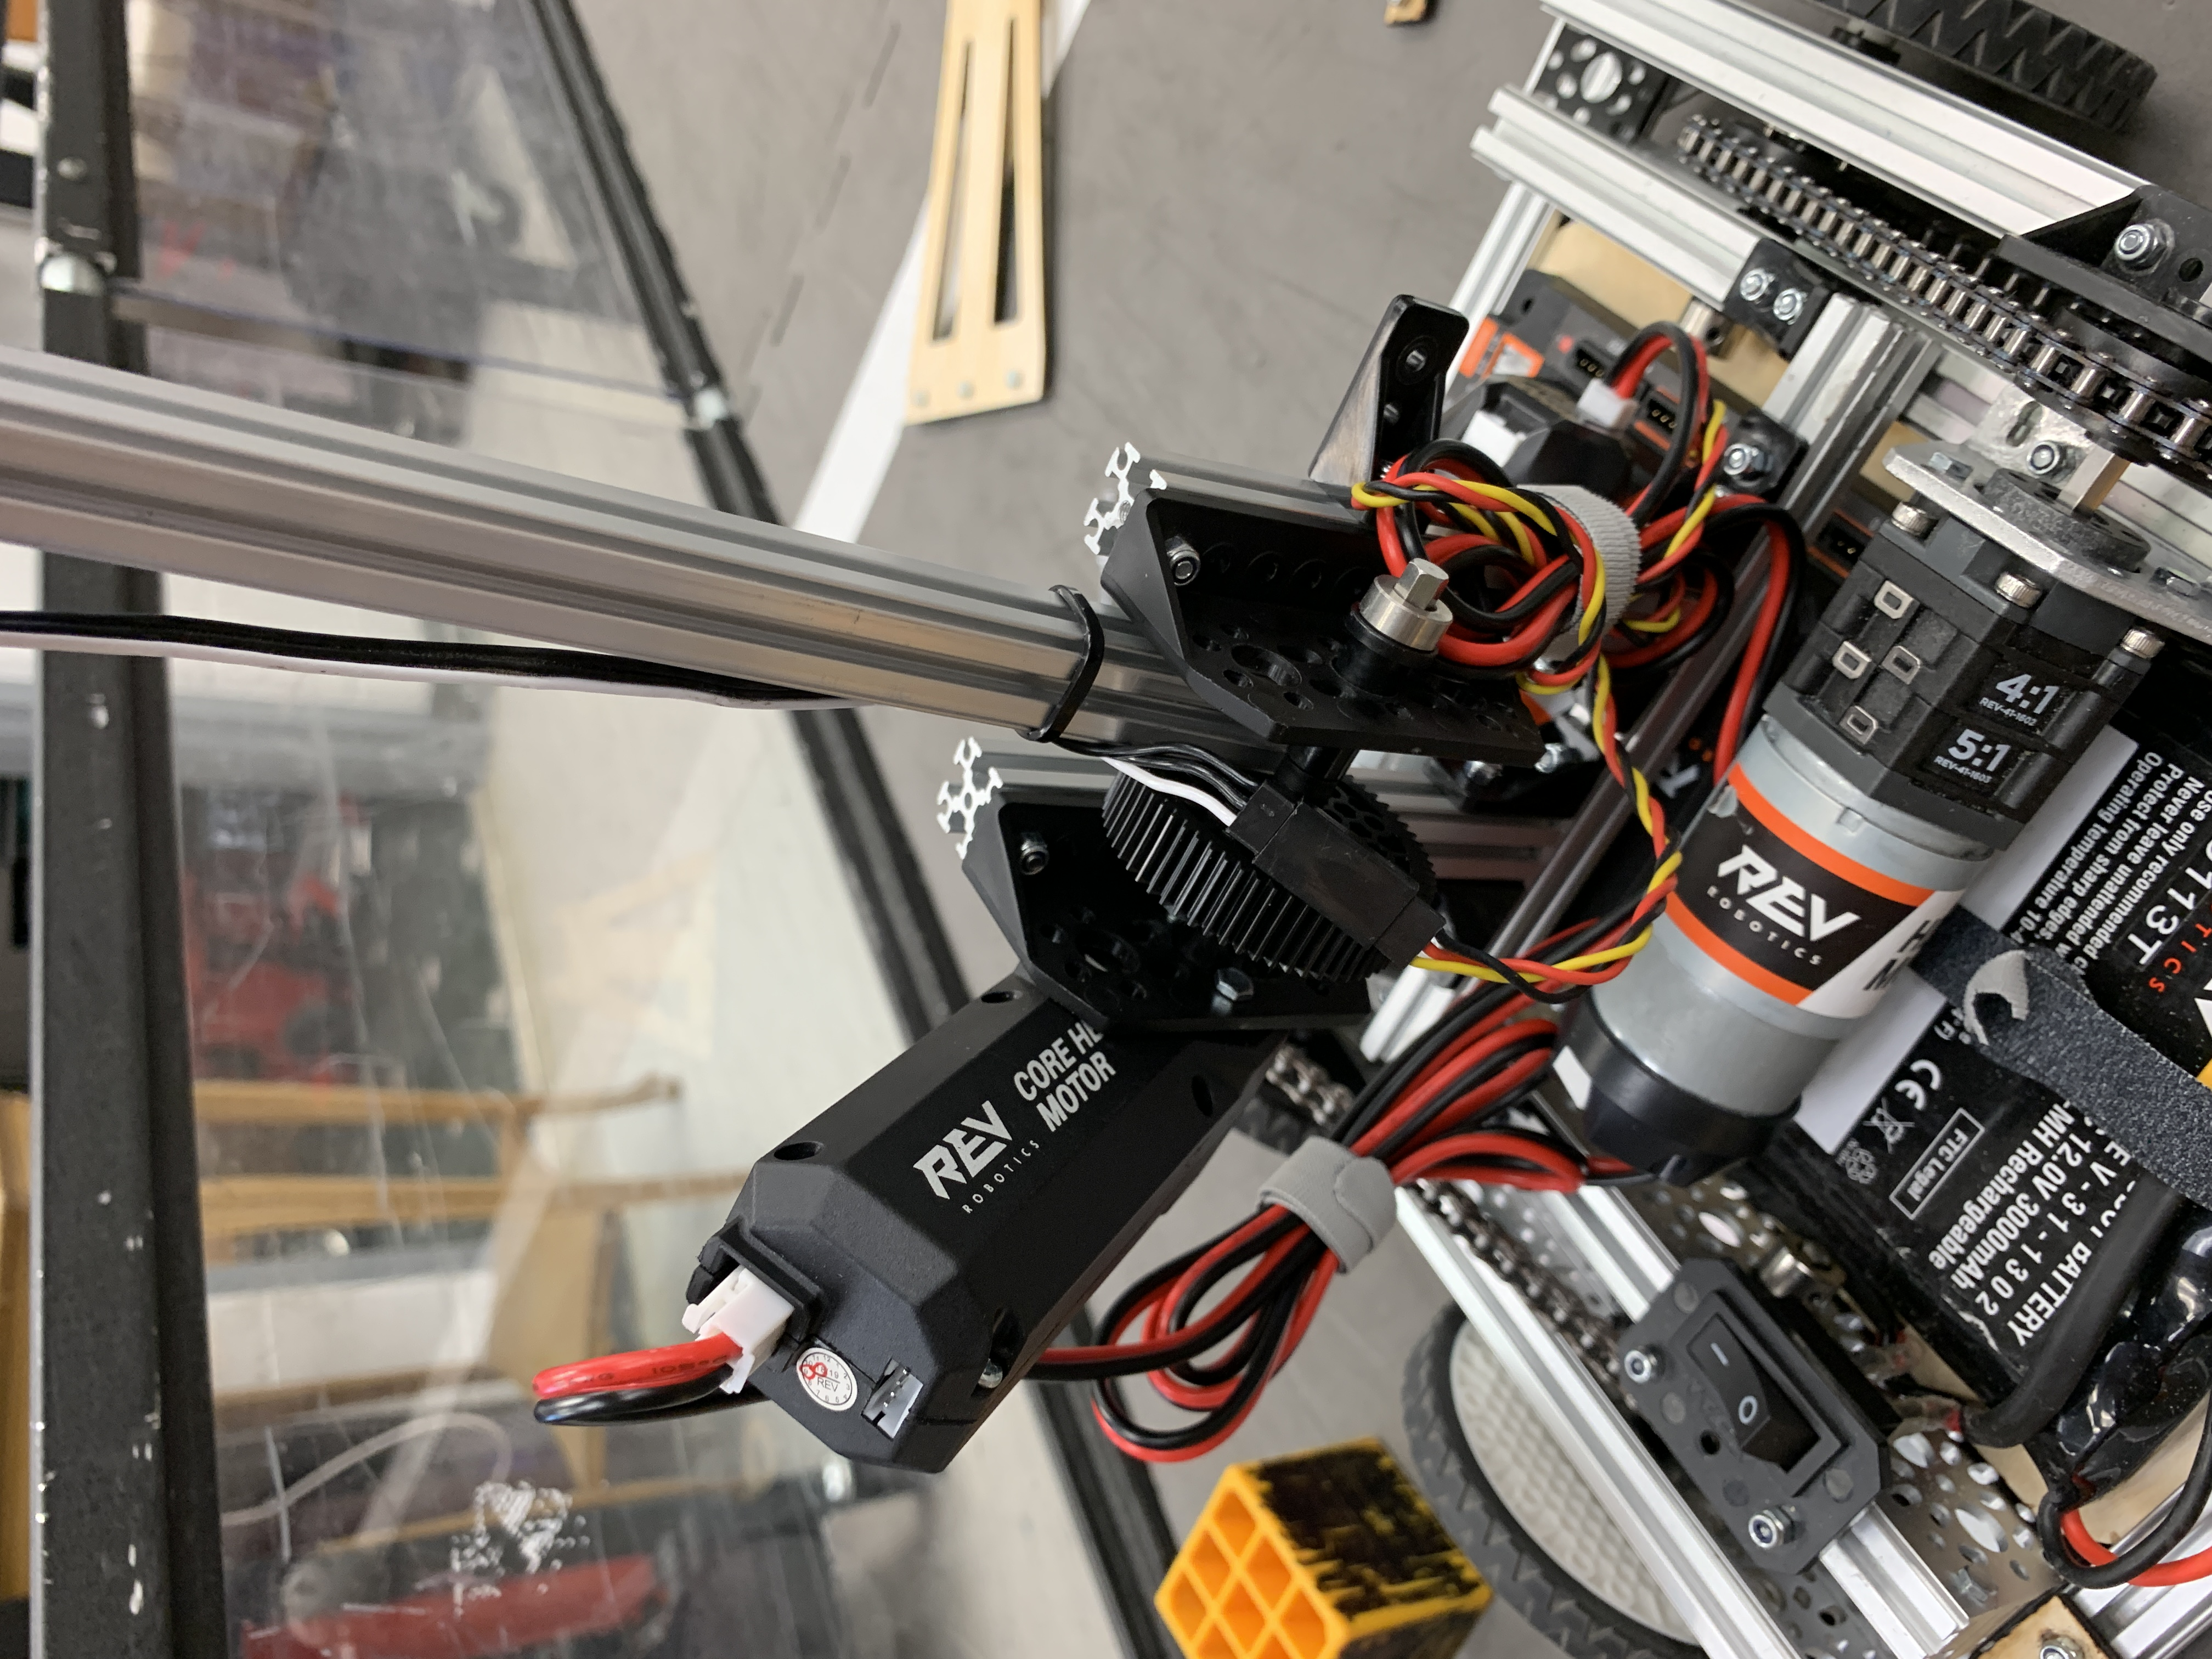
\includegraphics[width=0.8\textwidth]{Meetings/October/10-07-21/10-7-21_Hardware_Figure3 - Nathan Forrer.JPG}
  \caption{Our arm pivot mechanism.}
  \label{fig:pic3}
\end{minipage}%
\hfill%
\begin{minipage}[b]{.50\textwidth}
  \centering
  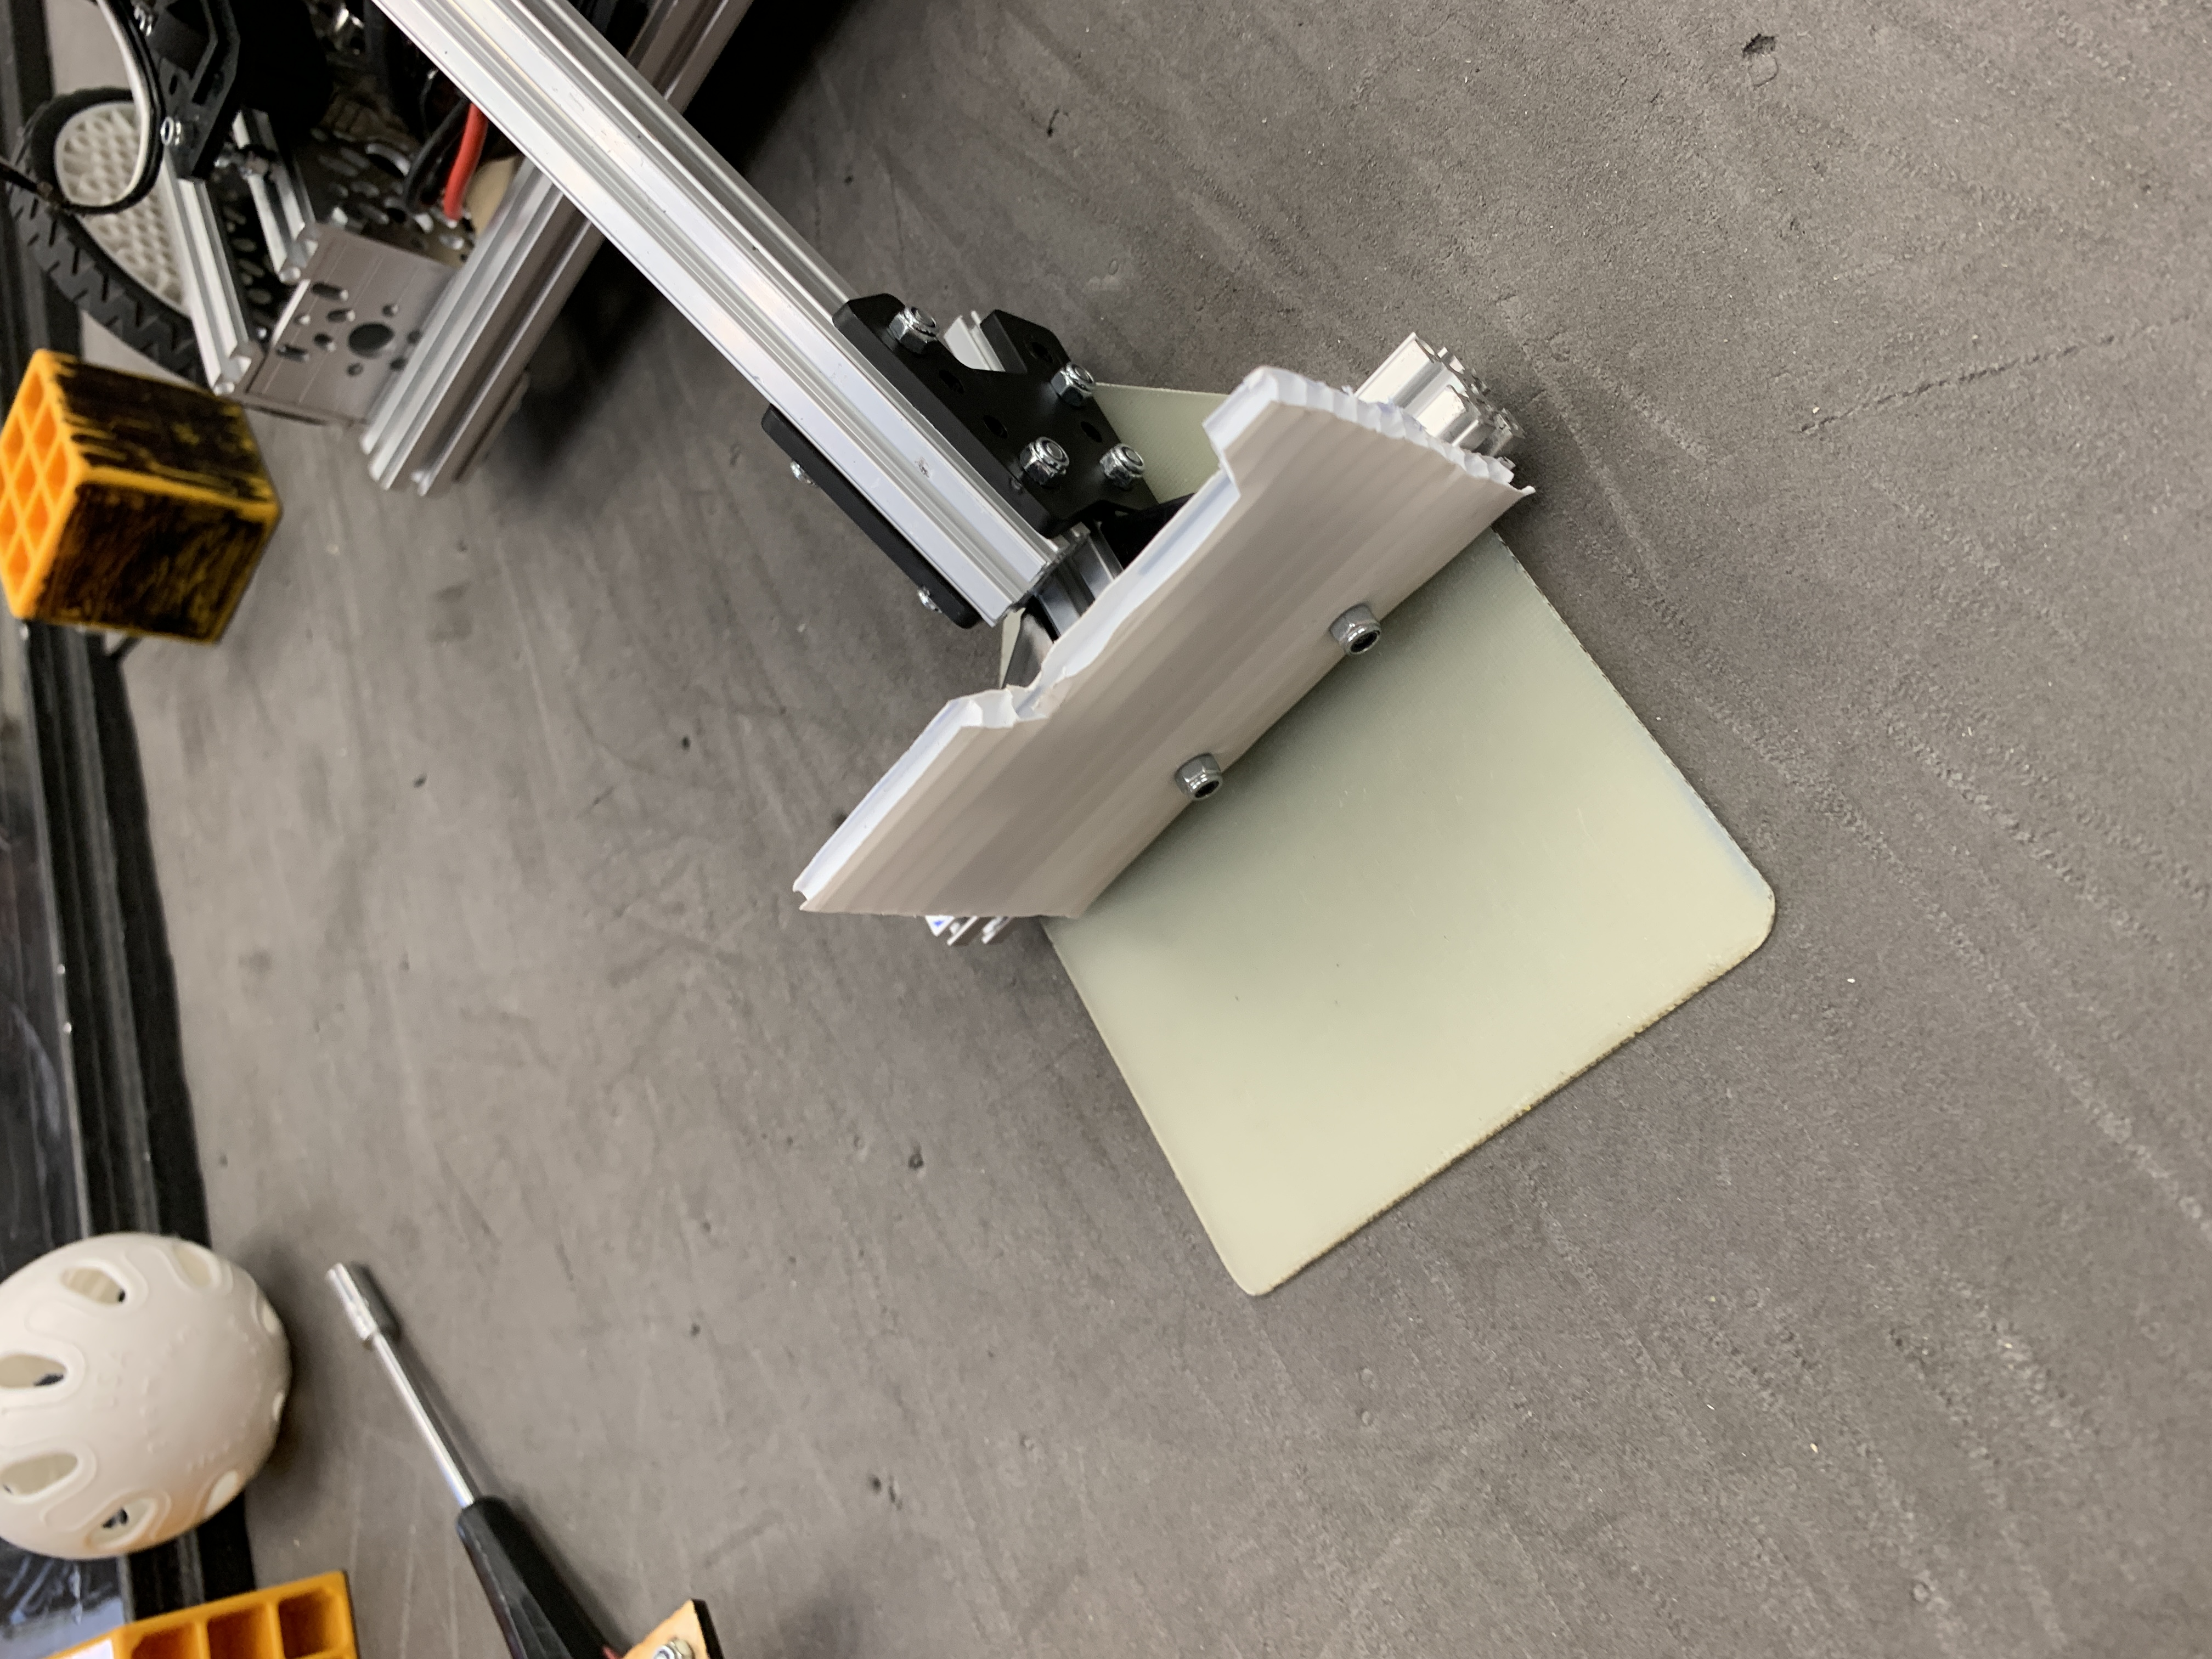
\includegraphics[width=0.8\textwidth]{Meetings/October/10-07-21/10-7-21_Hardware_Figure4 - Nathan Forrer.JPG}
  \caption{The first piece of our intake.}
  \label{fig:pic4}
\end{minipage}
\end{figure}